\documentclass[12pt]{article}

\usepackage{graphicx}
\usepackage[margin=1.0in]{geometry}
\usepackage{amsmath}
\usepackage{cases}
\usepackage{amsfonts}
\usepackage{amssymb}
\usepackage{grffile}
\usepackage{setspace}
\usepackage{listings}

\setlength\parindent{0pt}

\author{Xiaohui Chen \\EID: xc2388}
\title{PHY 362K Homework 5}

\begin{document}
\maketitle

\begin{spacing}{2.0}


\section{} %1

\subsection*{(a)}

According to Problem 3 in Homework 4, the matrix of $\vec{l} \cdot \vec{s}$ generated by uncoupled basis is:

$\left(
\begin{array}{cccccccc}
0 & 0 & 0 & 0 & 0 & 0 & 0 & 0 \\
0 & 0 & 0 & 0 & 0 & 0 & 0 & 0 \\
0 & 0 & \frac{\hbar^2}{2} & 0 & 0 & 0 & 0 & 0 \\
0 & 0 & 0 & -\frac{\hbar^2}{2} & \frac{\hbar^2}{\sqrt{2}} & 0 & 0 & 0 \\
0 & 0 & 0 & \frac{\hbar^2}{\sqrt{2}} & 0 & 0 & 0 & 0 \\
0 & 0 & 0 & 0 & 0 & 0 & \frac{\hbar^2}{\sqrt{2}} & 0 \\
0 & 0 & 0 & 0 & 0 & \frac{\hbar^2}{\sqrt{2}} & -\frac{\hbar^2}{2} & 0 \\
0 & 0 & 0 & 0 & 0 & 0 & 0 & \frac{\hbar^2}{2}
\end{array}
\right)
$

Let $\lambda$ be the eigenvalue and $c$ be eigenvectors

Using Mathematica, the eigenvalue and the corresponding eigenvectors are:

\end{spacing}

\begin{spacing}{1.5}

$\lambda_1=-\hbar ^2$,
$c_1=\left(
\begin{array}{c}
 0 \\
 0 \\
 0 \\
 0 \\
 0 \\
 -\frac{1}{\sqrt{3}} \\
 \sqrt{\frac{2}{3}} \\
 0 \\
\end{array}
\right)$;
$\lambda_2=-\hbar ^2$,
$c_2=\left(
\begin{array}{c}
 0 \\
 0 \\
 0 \\
 -\sqrt{\frac{2}{3}} \\
 \frac{1}{\sqrt{3}} \\
 0 \\
 0 \\
 0 \\
\end{array}
\right)$;
$\lambda_3=\frac{\hbar ^2}{2}$,
$c_3=\left(
\begin{array}{c}
 0 \\
 0 \\
 0 \\
 0 \\
 0 \\
 0 \\
 0 \\
 1 \\
\end{array}
\right)$;
$\lambda_4=\frac{\hbar ^2}{2}$,
$c_4=\left(
\begin{array}{c}
 0 \\
 0 \\
 0 \\
 0 \\
 0 \\
 \sqrt{\frac{2}{3}} \\
 \frac{1}{\sqrt{3}} \\
 0 \\
\end{array}
\right)$;
$\lambda_5=\frac{\hbar ^2}{2}$,
$c_5=\left(
\begin{array}{c}
 0 \\
 0 \\
 0 \\
 \frac{1}{\sqrt{3}} \\
 \sqrt{\frac{2}{3}} \\
 0 \\
 0 \\
 0 \\
\end{array}
\right)$;
$\lambda_6=\frac{\hbar ^2}{2}$,
$c_6=\left(
\begin{array}{c}
 0 \\
 0 \\
 1 \\
 0 \\
 0 \\
 0 \\
 0 \\
 0 \\
\end{array}
\right)$;
$\lambda_7=0$,
$c_7=\left(
\begin{array}{c}
 0 \\
 1 \\
 0 \\
 0 \\
 0 \\
 0 \\
 0 \\
 0 \\
\end{array}
\right)$;
$\lambda_8=0$,
$c_8=\left(
\begin{array}{c}
 1 \\
 0 \\
 0 \\
 0 \\
 0 \\
 0 \\
 0 \\
 0 \\
\end{array}
\right)$

\end{spacing}

\begin{spacing}{2.0}

The Mathematica code for this part is shown below:

\begin{lstlisting}[language=Mathematica,breaklines=true,frame=single]
m:={{0, 0, 0, 0, 0, 0, 0, 0}, {0, 0, 0, 0, 0, 0, 0, 0},
{0, 0, \[HBar]^2/ 2, 0, 0, 0, 0, 0},
{0, 0, 0, -(\[HBar]^2/2), \[HBar]^2/Sqrt[2], 0, 0, 0},
{0, 0, 0, \[HBar]^2/Sqrt[2], 0, 0, 0, 0},
{0, 0, 0, 0, 0, 0, \[HBar]^2/Sqrt[2], 0},
{0, 0, 0, 0, 0, \[HBar]^2/Sqrt[2], -(\[HBar]^2/2), 0},
{0, 0, 0, 0, 0, 0, 0, \[HBar]^2/2}}
eigen:=Eigensystem[m]
values:=Part[eigen,1]
vectors:=Part[eigen,2]
Do[Print[TeXForm[Part[values,i]]],{i,1,8}]
Do[Print[TeXForm[Normalize[Part[vectors,i]]//MatrixForm]],{i,1,8}]
\end{lstlisting}

\subsection*{(b)}

The matrix of $\vec{l} \cdot \vec{s}$ generated by coupled basis is:

$\left(
\begin{array}{cccccccc}
 0 & 0 & 0 & 0 & 0 & 0 & 0 & 0 \\
 0 & 0 & 0 & 0 & 0 & 0 & 0 & 0 \\
 0 & 0 & -\hbar ^2 & 0 & 0 & 0 & 0 & 0 \\
 0 & 0 & 0 & -\hbar ^2 & 0 & 0 & 0 & 0 \\
 0 & 0 & 0 & 0 & \frac{1}{2}\hbar ^2 & 0 & 0 & 0 \\
 0 & 0 & 0 & 0 & 0 & \frac{1}{2}\hbar ^2 & 0 & 0 \\
 0 & 0 & 0 & 0 & 0 & 0 & \frac{1}{2}\hbar ^2 & 0 \\
 0 & 0 & 0 & 0 & 0 & 0 & 0 & \frac{1}{2}\hbar ^2 \\
\end{array}
\right)$

Since the elements not in the diagonal are 0, the eigenvalues are the elements in the diagonal

By inspecting $\lambda_1,\ldots,\lambda_8$ in part (a), we can know that each $\lambda$ corresponds to one element of the diagonal in the above matrix

Therefore,

$c_1$ corresponds to $-\frac{1}{\sqrt{3}} |2,1,0,\frac{1}{2} \rangle + \sqrt{\frac{2}{3}}|2,1,1,-\frac{1}{2}\rangle$ for the uncoupled basis, which is equivalent to $|2,1,\frac{1}{2},\frac{1}{2} \rangle$ for the coupled basis. The corresponding eigenvalues in both matrices are both $-\hbar ^2$\\

$c_2$ corresponds to $-\sqrt{\frac{2}{3}} |2,1,-1,\frac{1}{2} \rangle + \frac{1}{\sqrt{3}} |2,1,0,-\frac{1}{2}\rangle$ for the uncoupled basis, which is equivalent to $|2,1,\frac{1}{2},-\frac{1}{2} \rangle$ for the coupled basis. The corresponding eigenvalues in both matrices are both $-\hbar ^2$\\

$c_3$ corresponds to $ |2,1,1,\frac{1}{2} \rangle$ for the uncoupled basis, which is equivalent to $|2,1,\frac{3}{2},\frac{3}{2} \rangle$ for the coupled basis. The corresponding eigenvalues in both matrices are both $\frac{\hbar^2}{2}$\\

$c_4$ corresponds to $\sqrt{\frac{2}{3}} |2,1,0,\frac{1}{2} \rangle + \frac{1}{\sqrt{3}}|2,1,1,-\frac{1}{2}\rangle$ for the uncoupled basis, which is equivalent to $|2,1,\frac{3}{2},\frac{1}{2} \rangle$ for the coupled basis. The corresponding eigenvalues in both matrices are both $\frac{\hbar^2}{2}$\\

$c_5$ corresponds to $\frac{1}{\sqrt{3}} |2,1,-1,\frac{1}{2} \rangle + \sqrt{\frac{2}{3}} |2,1,0,-\frac{1}{2}\rangle$ for the uncoupled basis, which is equivalent to $|2,1,\frac{3}{2},-\frac{1}{2} \rangle$ for the coupled basis. The corresponding eigenvalues in both matrices are both $\frac{\hbar^2}{2}$\\

$c_6$ corresponds to $ |2,1,-1,-\frac{1}{2} \rangle$ for the uncoupled basis, which is equivalent to $|2,1,\frac{3}{2},-\frac{3}{2} \rangle$ for the coupled basis. The corresponding eigenvalues in both matrices are both $\frac{\hbar^2}{2}$\\

$c_7$ corresponds to $|2,0,0,\frac{1}{2} \rangle$ for the uncoupled basis, which is equivalent to $|2,0,\frac{1}{2},\frac{1}{2} \rangle$ for the coupled basis. The corresponding eigenvalues in both matrices are both $0$\\

$c_8$ corresponds to $|2,0,0,-\frac{1}{2} \rangle$ for the uncoupled basis, which is equivalent to $|2,0,\frac{1}{2},-\frac{1}{2} \rangle$ for the coupled basis. The corresponding eigenvalues in both matrices are both $0$

We therefore conclude that each eigenvector in part (b) corresponds to a vector in coupled basis. Also, the corresponding eigenvalues are the same

\subsection*{(c)}

According to part (b), we can write the vector in coupled basis and the linear combination of vectors in uncoupled basis as $|n,l,j,m_j \rangle = \sum\limits_{i} a_i |n,l,m_l,m_s \rangle_i$, where $a_i$ represents the coefficient

$|2,1,\frac{1}{2},\frac{1}{2} \rangle = -\frac{1}{\sqrt{3}} |2,1,0,\frac{1}{2} \rangle + \sqrt{\frac{2}{3}}|2,1,1,-\frac{1}{2}\rangle$\\

$|2,1,\frac{1}{2},-\frac{1}{2} \rangle = -\sqrt{\frac{2}{3}} |2,1,-1,\frac{1}{2} \rangle + \frac{1}{\sqrt{3}} |2,1,0,-\frac{1}{2}\rangle$\\

$|2,1,\frac{3}{2},\frac{3}{2} \rangle = |2,1,1,\frac{1}{2} \rangle$\\

$|2,1,\frac{3}{2},\frac{1}{2} \rangle = \sqrt{\frac{2}{3}} |2,1,0,\frac{1}{2} \rangle + \frac{1}{\sqrt{3}}|2,1,1,-\frac{1}{2}\rangle$\\

$|2,1,\frac{3}{2},-\frac{1}{2} \rangle = \frac{1}{\sqrt{3}} |2,1,-1,\frac{1}{2} \rangle + \sqrt{\frac{2}{3}} |2,1,0,-\frac{1}{2}\rangle$\\

$|2,1,\frac{3}{2},-\frac{3}{2} \rangle = |2,1,-1,-\frac{1}{2} \rangle$\\

$|2,0,\frac{1}{2},\frac{1}{2} \rangle = |2,0,0,\frac{1}{2} \rangle$\\

$|2,0,\frac{1}{2},-\frac{1}{2} \rangle = |2,0,0,-\frac{1}{2} \rangle$

With the equations above, we can write the four uncoupled vectors as linear combinations of coupled vectors: $ |n,l,m_l,m_s \rangle = \sum\limits_{i} b_i  |n,l,j,m_j \rangle_i$, where $b_i$ represents the coefficient

$|2,1,0,\frac{1}{2} \rangle= \sqrt{\frac{2}{3}} |2,1,\frac{3}{2}, \frac{1}{2} \rangle - \frac{1}{\sqrt{3}} |2,1,\frac{1}{2}, \frac{1}{2} \rangle$\\

$|2,1,1,-\frac{1}{2} \rangle= \frac{1}{\sqrt{3}}  |2,1,\frac{3}{2}, \frac{1}{2} \rangle + \sqrt{\frac{2}{3}} |2,1,\frac{1}{2}, \frac{1}{2} \rangle$\\

$|2,1,-1,\frac{1}{2} \rangle= \frac{1}{\sqrt{3}} |2,1,\frac{3}{2}, -\frac{1}{2} \rangle -  \sqrt{\frac{2}{3}} |2,1,\frac{1}{2}, -\frac{1}{2} \rangle$\\

$|2,1,0,-\frac{1}{2} \rangle= \sqrt{\frac{2}{3}} |2,1,\frac{3}{2}, -\frac{1}{2} \rangle +   \frac{1}{\sqrt{3}} |2,1,\frac{1}{2}, -\frac{1}{2} \rangle$\\


By checking the Clebsch-Gordant coefficient table, I can verify that the coefficients in the four linear combinations above corresponds with the Clebsch-Gordant coefficients

\section{} %2

\subsection*{(a)}

The operator $H_{kin}$ is diagonal

$H_{kin}|2,1,-1,\frac{1}{2}\rangle = -\frac{\alpha^2}{4} |E_2^{(0)}| \left(\frac{2}{1+\frac{1}{2}}-\frac{3}{4} \right) |2,1,-1,\frac{1}{2}\rangle = -\frac{7\alpha^2}{48} |E_2^{(0)}| |2,1,-1,\frac{1}{2}\rangle$

$H_{kin}|2,1,0,-\frac{1}{2}\rangle= -\frac{\alpha^2}{4} |E_2^{(0)}| \left(\frac{2}{1+\frac{1}{2}}-\frac{3}{4} \right) |2,1,0,-\frac{1}{2}\rangle = -\frac{7\alpha^2}{48} |E_2^{(0)}| |2,1,0,-\frac{1}{2}\rangle$

Therefore $H_{kin}= \left(
\begin{array}{cc}
-\frac{7\alpha^2}{48} |E_2^{(0)}| & 0 \\
0 & -\frac{7\alpha^2}{48} |E_2^{(0)}|
\end{array}
\right)
$\\

The operator $H_D$ is also diagonal

$H_{D}|2,1,-1,\frac{1}{2}\rangle = 0 |2,1,-1,\frac{1}{2}\rangle$

$H_{D}|2,1,0,-\frac{1}{2}\rangle = 0 |2,1,0,-\frac{1}{2}\rangle$

Therefore $H_{D}= \left(
\begin{array}{cc}
0 & 0 \\
0 & 0
\end{array}
\right)
$\\

We already know that $\vec{l} \cdot \vec{s}= \left(
\begin{array}{cc}
-\frac{\hbar^2}{2} & \frac{\hbar^2}{\sqrt{2}}\\
\frac{\hbar^2}{\sqrt{2}} & 0
\end{array}
\right)$

We also know that

$\frac{1}{r^3}|2,1,-1,\frac{1}{2}\rangle = \frac{1}{2^3\left(1+\frac{1}{2}\right)2a_0^3} |2,1,-1,\frac{1}{2}\rangle= \frac{1}{24 a_0^3} |2,1,-1,\frac{1}{2}\rangle$

$\frac{1}{r^3}|2,1,0,-\frac{1}{2}\rangle = \frac{1}{2^3\left(1+\frac{1}{2}\right)2a_0^3} |2,1,0,-\frac{1}{2}\rangle= \frac{1}{24 a_0^3} |2,1,0,-\frac{1}{2}\rangle$

Therefore operator $\frac{1}{r^3}$ is diagonal

Since $H_{SO}= \left( \frac{e^2}{4\pi \epsilon_0}\right) \left(\frac{1}{2m_e^2 c^2} \right) \frac{\vec{l} \cdot \vec{s}}{r^3} $

Since $|E_2^{(0)}|=\frac{1}{8}\alpha^2m_ec^2 $, $\alpha=\frac{e^2}{4\pi \epsilon_0 c}$ and $a_0= \frac{4\pi\epsilon_0\hbar^2}{m_e e^2}= \frac{1}{\alpha} \frac{\hbar^2}{m_e c}$

$H_{SO}= \left( \frac{e^2}{4\pi \epsilon_0}\right) \left(\frac{1}{2m_e^2 c^2} \right) \frac{1}{24 a_0^3} \left(
\begin{array}{cc}
-\frac{\hbar^2}{2} & \frac{\hbar^2}{\sqrt{2}}\\
\frac{\hbar^2}{\sqrt{2}} & 0
\end{array}
\right)= \frac{\alpha^2|E_2^{(0)}|}{6} \left(
\begin{array}{cc}
-\frac{1}{2} & \frac{1}{\sqrt{2}}\\
\frac{1}{\sqrt{2}} & 0
\end{array}
\right)$

$\therefore H_{fs}=H_{kin}+H_{SO}+H_{D}= $

$\left(
\begin{array}{cc}
-\frac{7\alpha^2}{48} |E_2^{(0)}| & 0 \\
0 & -\frac{7\alpha^2}{48} |E_2^{(0)}|
\end{array}
\right) +
\frac{\alpha^2|E_2^{(0)}|}{6} \left(
\begin{array}{cc}
-\frac{1}{2} & \frac{1}{\sqrt{2} }\\
\frac{1}{\sqrt{2}} & 0
\end{array}
\right) +
\left(
\begin{array}{cc}
0 & 0 \\
0 & 0
\end{array}
\right)
= $

$|E_2^{(0)}| \left(
\begin{array}{cc}
-\frac{11\alpha^2}{48} & \frac{\alpha^2}{6\sqrt{2}} \\
\frac{\alpha^2}{6\sqrt{2}} & -\frac{7\alpha^2}{48}
\end{array}
\right)$

The operator $H_z$ is diagonal and $H_z=\mu_B B \left( \frac{l_z+2s_z}{\hbar} \right)$

$H_{z}|2,1,-1,\frac{1}{2}\rangle = \mu_B B \hbar \left( \frac{-1+1}{\hbar} \right) |2,1,-1,\frac{1}{2}\rangle = 0$

$H_{z}|2,1,0,-\frac{1}{2}\rangle = \mu_B B \hbar \left( \frac{0-1}{\hbar} \right) |2,1,0,-\frac{1}{2}\rangle = -\mu_B B |2,1,0,-\frac{1}{2}\rangle$

Therefore the matrix $H_z= \left(
\begin{array}{cc}
0 & 0\\
0 & -\mu_B B
\end{array}
\right)$

Therefore the perturbed Hamiltonian is $H'= \left(
\begin{array}{cc}
\frac{-11\alpha^2 |E_2^{(0)}|}{48} & \frac{\alpha^2 |E_2^{(0)}|}{6\sqrt{2}} \\
\frac{\alpha^2 |E_2^{(0)}|}{6\sqrt{2}} & \frac{-7\alpha^2 |E_2^{(0)}|}{48} -\frac{\mu_B B}{\hbar}
\end{array}
\right)$

\subsection*{(b)}

When $B=0$, we can know that $H'= \left(
\begin{array}{cc}
\frac{-11\alpha^2 |E_2^{(0)}|}{48} & \frac{\alpha^2 |E_2^{(0)}|}{6\sqrt{2}} \\
\frac{\alpha^2 |E_2^{(0)}|}{6\sqrt{2}} & \frac{-7\alpha^2 |E_2^{(0)}|}{48}
\end{array}
\right)$

Using Mathematica to diagonalize $H'$, we get

$H'= \left(
\begin{array}{cc}
-\frac{5\alpha^2 |E_2^{(0)}| }{16} & 0 \\
0 & -\frac{1 \alpha^2 |E_2^{(0)}|}{16 }
\end{array}
\right)= 
\left(
\begin{array}{cc}
\frac{5\alpha^2 |E_2^{(0)}| }{16} & 0 \\
0 & \frac{1 \alpha^2 |E_2^{(0)}|}{16 }
\end{array}
\right)$

When $j=\frac{3}{2}$, $\langle H_{fs1} \rangle = -\frac{\alpha^2}{4}|E_2^{(0)}| \left[ \frac{2}{\frac{3}{2}+ \frac{1}{2}} - \frac{3}{4} \right]= -\frac{\alpha^2|E_2^{(0)}|}{16} $

When $j=\frac{1}{2}$, $\langle H_{fs2} \rangle = -\frac{\alpha^2}{4}|E_2^{(0)}| \left[ \frac{2}{\frac{1}{2}+ \frac{1}{2}} - \frac{3}{4} \right]= -\frac{5\alpha^2|E_2^{(0)}|}{16} $

The values of $\langle H_{fs1} \rangle$ and $\langle H_{fs2} \rangle$ above match the diagonal elements of the diagonal matrix. Therefore the fine structure matrix is correct

The Mathematica used in this part is shown below:

\begin{lstlisting}[language=Mathematica,breaklines=true,frame=single]
Clear[a]
H' := {{-(11*a^2*En)/
    48, (a^2*En)/(6*Sqrt[2])}, {(a^2*En)/(6*Sqrt[2]), -(7*a^2*En)/48}}
JordanDecomposition[H']
\end{lstlisting}

\subsection*{(c)}

We know that $H_{fs}= \left(
\begin{array}{cc}
\frac{-11\alpha^2 |E_2^{(0)}|}{48} & \frac{\alpha^2 |E_2^{(0)}|}{6\sqrt{2}} \\
\frac{\alpha^2 |E_2^{(0)}|}{6\sqrt{2}} & \frac{-7\alpha^2 |E_2^{(0)}|}{48}
\end{array}
\right)$ and $H_Z= \left(
\begin{array}{cc}
0 & 0\\
0 & -\mu_B B
\end{array}
\right)$

Using Mathematica, we get the Frobenius magnitude of $H_{fs}$ is $\frac{1}{8} \sqrt{\frac{13}{2}} a_0^2 |E_2^{(0)}|$ and the magnitude of $H_Z$ is simply $\mu_B B$

$\therefore B_{int} = \frac{1}{8 \mu_B} \sqrt{\frac{13}{2}} a_0^2 |E_2^{(0)}| = 0.995593 T$

The Mathematica code used in this part is shown below:

\begin{lstlisting}[language=Mathematica,breaklines=true,frame=single]
En := (13.6/4)*1.6*10^(-19)
a := 7.2974*10^(-3)
mu := 9.273*10^(-24)
Simplify[Solve[mu*B == 1/8 Sqrt[13/2] a^2 En, B],
 B \[Element] Reals && B > 0]
\end{lstlisting}

\subsection*{(d)}

The perturbed Hamiltonian is $H'= \left(
\begin{array}{cc}
\frac{-11\alpha^2 |E_2^{(0)}|}{48} & \frac{\alpha^2 |E_2^{(0)}|}{6\sqrt{2}} \\
\frac{\alpha^2 |E_2^{(0)}|}{6\sqrt{2}} & \frac{-7\alpha^2 |E_2^{(0)}|}{48} -\frac{\mu_B B}{\hbar}
\end{array}
\right)$

Diagonalize the matrix, we get 

$H'= \left(
\begin{array}{cc}
f(B) & 0\\
0 & g(B)
\end{array}
\right)$

Where $f(B)=\frac{1}{48} \left(-9 \alpha^2 |E_2^{(0)}|-24\mu_B B-\sqrt{36 \alpha^4|E_2^{(0)}|^2-96 \alpha^2 B|E_2^{(0)}|\mu_B+ 576B^2\mu_B^2 }\right)$ ,

$g(B)=\frac{1}{48} \left(-9 \alpha^2 |E_2^{(0)}|-24\mu_B B+\sqrt{36 \alpha^4|E_2^{(0)}|^2-96 \alpha^2 B|E_2^{(0)}|\mu_B+ 576B^2\mu_B^2 }\right)$

\begin{figure}
  \centering
  % Requires \usepackage{graphicx}
  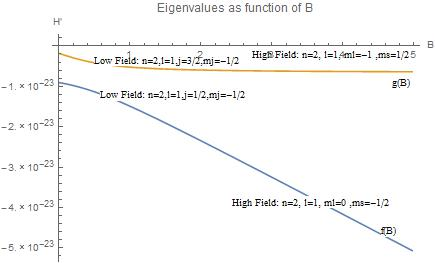
\includegraphics[width=6in]{out1}\\
  \caption{Plot of $f(B)$ and $g(B)$ vs. $B$}\label{out1}
\end{figure}

The plot of $f(B)$ and $g(B)$ is shown in Figure \ref{out1}

The Mathematica code I used in this part is shown below:

\begin{lstlisting}[language=Mathematica,breaklines=true,frame=single]
Clear[En]
Clear[a]
Clear[mu]
H := {{-(11*a^2*En)/
    48, (a^2*En)/(6*Sqrt[2])}, {(a^2*En)/(6*Sqrt[2]), -(7*a^2*En)/
     48 - mu*B}}
JordanDecomposition[H]
f := (1/48) (-9 a^2 En - 24 B mu -
    2 Sqrt[3] Sqrt[3 a^4 En^2 - 8 a^2 B En mu + 48 B^2 mu^2])
g := (1/48) (-9 a^2 En - 24 B mu +
    2 Sqrt[3] Sqrt[3 a^4 En^2 - 8 a^2 B En mu + 48 B^2 mu^2])
En := (13.6/4)*1.6*10^(-19)
a := 7.2974*10^(-3)
mu := 9.273*10^(-24)
Plot[{f, g}, {B, 0, 5*0.995592544948975`},
 PlotLabel -> "Eigenvalues as function of B",
 AxesLabel -> {"B", "H'"}, PlotLegends -> {"f(B)", "g(B)"}]
\end{lstlisting}

\subsection*{(e)}

We know that

$f(B)=\frac{1}{48} \left(-9 \alpha^2 |E_2^{(0)}|-24\mu_B B-\sqrt{36 \alpha^4|E_2^{(0)}|^2-96 \alpha^2 B|E_2^{(0)}|\mu_B+ 576B^2\mu_B^2 }\right)$ ,

$g(B)=\frac{1}{48} \left(-9 \alpha^2 |E_2^{(0)}|-24\mu_B B+\sqrt{36 \alpha^4|E_2^{(0)}|^2-96 \alpha^2 B|E_2^{(0)}|\mu_B+ 576B^2\mu_B^2 }\right)$

When $B>>B_{int}$, the dominant term in the square root is $B^2$. We omit other terms expect for $B^2$ and $B$

Therefore $f(B)\approx -frac{1}{48}(-24\mu_B B -24\mu_B B)= -\mu_B B$

$g(B) \approx -frac{1}{48} (-24\mu_B B +24\mu_B B) = 0$

The expected value of $f(B)$ is $f(B)_{exp}= \mu_B *B * (0-2*1/2)=-\mu_B B$

The expected value of $g(B)$ is $g(B)_{exp}= \mu_B *B * (-1+2*1/2)=0$

By comparison, we know the expected values of the eigenvalues match the functions we obtained in part (d)

\subsection*{(f)}

We know that

$f(B)=\frac{1}{48} \left(-9 \alpha^2 |E_2^{(0)}|-24\mu_B B-\sqrt{36 \alpha^4|E_2^{(0)}|^2-96 \alpha^2 B|E_2^{(0)}|\mu_B+ 576B^2\mu_B^2 }\right)$ ,

$g(B)=\frac{1}{48} \left(-9 \alpha^2 |E_2^{(0)}|-24\mu_B B+\sqrt{36 \alpha^4|E_2^{(0)}|^2-96 \alpha^2 B|E_2^{(0)}|\mu_B+ 576B^2\mu_B^2 }\right)$

When $B<<B_{int}$, expand to power series, we get

$f(B)= -\frac{\mu_B }{3}B -\frac{5\alpha^2}{16} |E_2^{(0)}|$

$g(B)= -\frac{2\mu_B }{3}B -\frac{\alpha^2}{16} |E_2^{(0)}|$

$m_j=-\frac{1}{2}$ for both $f$ and $g$

From the above equations, we get $g_{jf}= \frac{2}{3}$ and $g_{jg}= \frac{4}{3}$

Since $g_j = \left[ 1+ \frac{j(j+1)-l(l+1)+3/4}{2j(j+1)} \right]$, we get that 

$\therefore g_{jf}=\left[ 1+ \frac{\frac{1}{2}(\frac{1}{2}+1)- 1(1+1)+3/4}{2\frac{1}{2}(\frac{1}{2}+1)} \right] = \frac{2}{3}$

$g_{jg}= \left[ 1+ \frac{\frac{3}{2}(\frac{3}{2}+1)- 1(1+1) +3/4}{2\frac{3}{2}(\frac{3}{2}+1)} \right]= \frac{3}{4}$

By comparison, we know that $g_{jf}$ and $g_{jg}$ agree with the general formula

The Mathematica code I used in this part is shown below:

\begin{lstlisting}[language=Mathematica,breaklines=true,frame=single]
Clear[En]
Clear[a]
Clear[mu]
Clear[B]
Simplify[Series[f, {B, 0, 1}],
 En \[Element] Reals && a \[Element] Reals && mu \[Element] Reals &&
  En > 0]
Simplify[Series[g, {B, 0, 1}],
 En \[Element] Reals && a \[Element] Reals && mu \[Element] Reals &&
  En > 0]
\end{lstlisting}


\section{} %3

\subsection*{(a)}

According to the problem, we can know that the perturbed Hamiltonian is $H'= e\mathcal{E}z$, the Bohr radius $a=0.529*10^{-10} m$

Since we need $n$ up to 4, we get

$|\psi_{100}^{(0)} \rangle= c_{210}|\psi_{210}\rangle + c_{310}|\psi_{210}\rangle + c_{410}|\psi_{210}\rangle$

$\therefore c_{210}= \frac{e\mathcal{E} \langle \psi_{210}^{(0)}|z| \psi_{100}^{(0)} \rangle}{E_1^{(0)} -E_2^{(0)}}= \frac{\mathcal{E}*\frac{128 \sqrt{2} a}{243}}{-10.2}= -3.09075*10^{-7}$

$\therefore c_{310}= \frac{e\mathcal{E} \langle \psi_{310}^{(0)}|z| \psi_{100}^{(0)} \rangle}{E_1^{(0)} -E_3^{(0)}}= \frac{\mathcal{E}*\frac{27 a}{64 \sqrt{2}}}{-12.0889}= -1.04431*10^{-7}$

$\therefore c_{410}= \frac{e\mathcal{E} \langle \psi_{410}^{(0)}|z| \psi_{100}^{(0)} \rangle}{E_1^{(0)} -E_4^{(0)}}= \frac{\mathcal{E}*\frac{6144 a}{15625 \sqrt{5}}}{-12.75}= -5.83689*10^{-8}$

The exact value of $E_{100}^{(0)}$ is $E_{100}^{(0)}= -(2.25)4\pi \epsilon_0a^3\mathcal{E}^2$

$E_{100}^{(2)}= \frac{e^2 \mathcal{E}^2 |\langle \psi_{210}^{(0)}|z| \psi_{100}^{(0)} \rangle|^2}{E_1^{(0)} -E_2^{(0)}} +
\frac{e^2 \mathcal{E}^2 |\langle \psi_{310}^{(0)}|z| \psi_{100}^{(0)} \rangle|^2}{E_1^{(0)} -E_3^{(0)}} +
\frac{e^2 \mathcal{E}^2 |\langle \psi_{410}^{(0)}|z| \psi_{100}^{(0)} \rangle|^2}{E_1^{(0)} -E_4^{(0)}}\approx -1.74601 4\pi \epsilon_0 a^3 \mathcal{E}^2 $

The difference between $-1.74601$ and $-2.25$ is small. Therefore with only three states, the second order energy is good enough

The mathematica code used in this part is shown below:

\begin{lstlisting}[language=Mathematica,breaklines=true,frame=single]
U[n_, l_, m_, r_, t_, phi_] :=
 Sqrt[(2/(n a))^3 ((n - l - 1)!/(2 n (n + l)!))]*
  Exp[-r/(n a)]*(2 r/(n a))^l*
  LaguerreL[n - l - 1, 2 l + 1, 2 r/(n a)]*
  SphericalHarmonicY[l, m, t, phi]

Simplify[Integrate[
  Conjugate[U[2, 1, 0, r, t, phi]]*U[1, 0, 0, r, t, phi]*r^3*Sin[t]*
   Cos[t], {r, 0, Infinity}, {t, 0, Pi}, {phi, 0, 2*Pi}],
 a \[Element] Reals && a > 0]

Simplify[Integrate[
  Conjugate[U[3, 1, 0, r, t, phi]]*U[1, 0, 0, r, t, phi]*r^3*Sin[t]*
   Cos[t], {r, 0, Infinity}, {t, 0, Pi}, {phi, 0, 2*Pi}],
 a \[Element] Reals && a > 0]

Simplify[Integrate[
  Conjugate[U[4, 1, 0, r, t, phi]]*U[1, 0, 0, r, t, phi]*r^3*Sin[t]*
   Cos[t], {r, 0, Infinity}, {t, 0, Pi}, {phi, 0, 2*Pi}],
 a \[Element] Reals && a > 0]

DeltaE[n_] := (-13.6 + (13.6/n^2))
DeltaE[2]
DeltaE[3]
DeltaE[4]

V := 80000
a := 0.529*10^(-10)

Clear[V]
Clear[a]
Energy[n_] := -2*(fourpi)*ep*a*
  V^2*((Simplify[
       Integrate[
        Conjugate[U[n, 1, 0, r, t, phi]]*U[1, 0, 0, r, t, phi]*r^3*
         Sin[t]*Cos[t], {r, 0, Infinity}, {t, 0, Pi}, {phi, 0, 2*Pi}],
        a \[Element] Reals && a > 0]^2)/(1 - (1/n^2)))

Energy[2] + Energy[3] + Energy[4]
\end{lstlisting}

\subsection*{(b)}

$E=-\frac{1}{2} \alpha \mathcal{E}^2 = -(2.250)4\pi\epsilon_0 a_0^3 \mathcal{E}^2$

$\therefore \frac{\alpha}{4\pi}= \frac{9}{2} a_0^3 \approx 6.66*10^{-31}$

Experimentally, the polarizability of hydrogen is given by $6.67*10^{-31}$. Therefore the calculated result is very accurate

\section{} %4

\subsection*{(a)}

The nuclear magnetic moment is given by $\mu_N= 5.0507*10^{-27} J/T$

$\mu_Z = g_I \mu_N \frac{I_z}{\hbar}= g_I \mu_N\frac{\hbar M_I}{\hbar}= g_I \mu_N= 0.8574*5.0507*10^{-27} J/T = 4.3304*10^{-27} J/T$

This matches the expected value $4.3307*10^{-27} J/T$

\subsection*{(b)}

The Hamiltonian due to Normal Zeeman effect is $H_z= -\mu_N g_I \frac{I_z}{\hbar}B $

$\therefore E_z= -\mu_N g_I M_I B$

We know that $B=1T$

Therefore $E_{z,M_I=0} = 0$, $E_{z,M_I=1} = -\mu_Z B= -4.3307*10^{-27} J$, $E_{z,M_I=-1}= \mu_Z B= 4.3307*10^{-27} J$

From $M_I=-1$ to $M_I=0$ or $M_I=0$ to $M_I=1$, the frequency of the photon emitted is $f=\frac{\Delta E}{h}= \frac{4.3307*10^{-27}}{6.63*10^{-34}} Hz = 6.532*10^{6} Hz$

\subsection*{(c)}

Since the electron in deuteron is in ground state, the Hamiltonian of Hyperfine energy only includes the term of Fermi contact

Therefore $H_{hy}= -\frac{\mu_0}{4\pi} \frac{8\pi}{3} \vec{\mu}_s\cdot \vec{\mu}_I \delta^3(\vec{r})$

$\vec{\mu}_s= -\mu_B g_e\frac{\vec{s}}{\hbar}$ and $\vec{\mu}_I = \mu_N g_I\frac{\vec{I}}{\hbar}$

Therefore $H_{hy}= \frac{\mu_0}{4\pi} \frac{8\pi}{3} \frac{\mu_B g_e\mu_N g_I}{\hbar^2} \vec{s} \cdot \vec{I} \delta^3(\vec{r})$

Let $\vec{F}= \vec{s}+\vec{I}$

$\therefore E_{hy}=\frac{\mu_0}{4\pi} \frac{8\pi}{3} \mu_B g_e\mu_N g_I|\psi_{100}(0)|^2 \frac{1}{2} (f(f+1)-s(s+1)-i(i+1))$ where $f=i+s= 1+\frac{1}{2}= \frac{3}{2}$

We know that the Bohr radius is $a_0=0.529*10^{-10}m $

$\Delta E = E_{hy}=\frac{\mu_0}{4\pi} \frac{8\pi}{3} \mu_B g_e\mu_N g_I \frac{1}{\pi a_0^3} \frac{1}{2} (\frac{3}{2}(\frac{3}{2}+1)- \frac{1}{2}(\frac{1}{2}+1)- 1(1+1)) = 7.23364*10^{-26} J$

$\therefore f_{trans}= \frac{\Delta E}{h}= 1.09105*10^8 Hz$

\end{spacing}
\end{document} 